\documentclass[11pt,a4paper]{article}

\usepackage[T1]{fontenc}
\usepackage[utf8]{inputenc}
\usepackage{lmodern}
\usepackage[margin=2.4cm]{geometry}
\usepackage{microtype}
\usepackage{booktabs}
\usepackage{multirow}
\usepackage{graphicx}
\usepackage{float}
\usepackage{subcaption}
\usepackage{amsmath}
\usepackage{siunitx}
\usepackage[dvipsnames]{xcolor}
\usepackage{tikz}
\usetikzlibrary{positioning,arrows.meta,decorations.pathreplacing}
\usepackage[colorlinks=true,allcolors=NavyBlue!70!black]{hyperref}

\sisetup{detect-all, group-minimum-digits=4}

\newcommand{\rmse}{nRMSE}
\newcommand{\best}[1]{\textbf{#1}}

\title{\bfseries MRIxFields 2026: Progress Report\\[0.3em]
\large Baselines, Representation Learning, and a Spectral View of Field-Strength Translation}
\author{Berkin Deniz Kahya \and Furkan Yüceyalçın \and Racha Badreddine \and Ahmet Zelka}
\date{}

\begin{document}
\maketitle

\begin{abstract}
\noindent
Report on the progress of the MRIxFields 2026 challenge, which asks for translation of brain MRI between
magnetic field strengths. In the baseline phase, we reproduced CUT, CycleGAN and StarGAN~v2 across all three
modalities and both paired tasks. Main finding of the phase is negative and consequential: an
\emph{identity} control that returns the input unchanged scores within noise of every trained baseline
on SSIM, Dice and volume consistency, and is beaten decisively only on \rmse{}. Consequently, published
baselines do not provide a meaningful baseline.

We also present a spectral analysis of the dataset, following Dieleman's observation~\cite{dieleman2024} that diffusion
models perform approximate autoregression in the frequency domain. Radially averaged power spectra of
axial slices follow an approximate power law $P(f) \propto f^{-\alpha}$, with exponents
larger than the $\alpha \approx 2$ found in natural
images~\cite{vanderschaaf1996,torralba2003,hyvarinen2009}. Crucially, the spectral gap between field
strengths is concentrated almost entirely at \SI{0.1}{\tesla}: from \SI{1.5}{\tesla} to \SI{7}{\tesla}
the exponents lie in a narrow, non-monotone band, and \SI{3}{\tesla} and \SI{5}{\tesla} sources already
match or exceed the \SI{7}{\tesla} target in high-frequency power. This explains the identity result
directly, since for most source field strengths there is little spectral content to add, and implies
that field-averaged metrics cannot distinguish a working model from a copy. Where a gap does exist,
translation is to first order a \emph{change in the slope of the power spectrum}, which is precisely
what a diffusion noise schedule controls. We argue this makes conditional diffusion, and in particular
frequency-aware formulations, a better-matched hypothesis class than the adversarial
baselines, and we outline the next phase of work.
\end{abstract}

\section{Introduction}

MRI Fields 2026 challenge concerns translation of brain MRI across magnetic field strengths.
Higher field strength provides signal-to-noise ratio, which raises spatial resolution and contrast;
the premise of the challenge is that a model might recover some of what a low-field scanner cannot
measure. Three tasks are defined over the field strengths $\{0.1, 1.5, 3, 5, 7\}\,\si{\tesla}$ and the
modalities $\{$T1W, T2W, T2FLAIR$\}$:

\begin{itemize}
  \item \textbf{Task 1}: translation from a given field strength to \SI{7}{\tesla}.
  \item \textbf{Task 2}: translation from \SI{0.1}{\tesla} to each higher field strength.
  \item \textbf{Task 3}: any-to-any translation across all field strengths with a single model.
\end{itemize}

Submissions are scored with \rmse{}, SSIM, LPIPS, and two segmentation-derived measures computed from
SynthSeg~\cite{billot2023synthseg} labels: Dice overlap and volume consistency. This report covers the work completed so far:
the baseline reproduction phase, an encoder-pretraining track, a conditional U-Net, and a new spectral
characterisation of the data that motivates our proposed direction.

\section{Data}
\label{sec:data}

The dataset is organised by split, modality and field strength. Volumes are
$364 \times 436 \times 364$, intensity-normalised to
$[0,1]$. Table~\ref{tab:data} gives the counts.

\begin{table}[t]
  \centering
  \small
  \caption{Volume counts per split. The retrospective training split is both far larger and
  substantially unbalanced across field strengths.}
  \label{tab:data}
  \begin{tabular}{llccccc c}
    \toprule
    Split & Modality & \SI{0.1}{\tesla} & \SI{1.5}{\tesla} & \SI{3}{\tesla} & \SI{5}{\tesla} & \SI{7}{\tesla} & Total \\
    \midrule
    \multirow{1}{*}{Validation (prospective)} & each & 3 & 3 & 3 & 3 & 3 & 45 \\
    \addlinespace
    Training (prospective) & each & 3 & 3 & 3 & 3 & 3 & 45 \\
    \addlinespace
    \multirow{3}{*}{Training (retrospective)}
      & T1W     & 100 & 104 & 143 & 121 & 235 & 703 \\
      & T2W     & 100 & 221 & 142 &  43 &  81 & 587 \\
      & T2FLAIR &  99 & 221 & 143 & 102 &  84 & 649 \\
    \bottomrule
  \end{tabular}
\end{table}

\subsection{The data is structurally unpaired across field strengths}
\label{sec:unpaired}

A property of the data release that affects our downstream analysis: \textbf{no subject appears at two
different field strengths}. Subject identifiers are allocated in blocks by field (in the
retrospective T1W split, identifiers $0001$--$0100$ are \SI{0.1}{\tesla}, $0101$ onward are
\SI{1.5}{\tesla}, $0329$ onward \SI{3}{\tesla}, and so on), and the pairwise intersection of
identifier sets across any two field strengths is empty. The same holds in the validation split.
Identifiers \emph{are} shared across modalities within a field strength, so modality is paired while
field strength is not.

Every comparison across
field strength, including the spectral comparison in Section~\ref{sec:spectral}, is a
between-subjects comparison, and anatomical variation is confounded with field strength. This is
tolerable at the retrospective sample sizes but not at the validation sizes, which is why we report the
spectral analysis primarily on the retrospective split.

\subsection{Note on background masking, zero background assumptions}
\label{sec:background}

Some volumes, most visibly T2W at \SI{1.5}{\tesla}, carry a small constant non-zero floor value,
($\approx 7\times10^{-5}$) across the entire field of view rather than exact zeros. Therefore, any foreground test,
\verb|voxel > 0| marks every slice as if it belongs to brain, including empty end slices. In the
first spectral pass, this allowed slices which are numerically meaningless, 
displacing the affected cell's mean log spectrum by roughly eight orders of
magnitude. Solution was to threshold relative to each volume's own intensity scale
($0.05 \times$ the $99.5$th percentile). This is noted down because the same pitfall can affect
any preprocessing or loss that assumes a zero background.

\section{Baseline phase}
\label{sec:baselines}

We reproduced the challenge baselines across modalities, distributing models across the team: CUT,
CycleGAN, StarGAN~v2, with per-model-per-modality evaluation. Table~\ref{tab:baselines} collects the
results, averaged across modalities.

\begin{table}[t]
  \centering
  \small
  \caption{Baseline results, mean across modalities. \textsc{input} is a control that returns the
  input volume unchanged, with no reconstruction of any kind.}
  \label{tab:baselines}
  \begin{tabular}{llccccc}
    \toprule
    Task & Model & \rmse{}~$\downarrow$ & SSIM~$\uparrow$ & LPIPS~$\downarrow$ & Dice~$\uparrow$ & Volume~$\uparrow$ \\
    \midrule
    Task 1 & CUT           & 0.3041 & \best{0.9053} & \best{0.0750} & 0.8542 & \best{0.8601} \\
    Task 1 & CycleGAN      & \best{0.3002} & 0.9052 & 0.0764 & 0.8498 & 0.8485 \\
    Task 1 & \textsc{input} (control) & 0.4085 & 0.8935 & 0.0897 & \best{0.8549} & 0.8586 \\
    \midrule
    Task 2 & CUT           & 0.2178 & \best{0.8657} & \best{0.1021} & \best{0.7664} & \best{0.7794} \\
    Task 2 & CycleGAN      & \best{0.2169} & 0.8639 & 0.1051 & 0.7102 & 0.7104 \\
    \midrule
    Task 3 & StarGAN~v2    & 0.3436 & 0.7397 & 0.1545 & --- & --- \\
    Task 3 & Conditional U-Net & \best{0.2364} & \best{0.9014} & \best{0.0890} & --- & --- \\
    \bottomrule
  \end{tabular}
\end{table}

\subsection{The identity control}

The \textsc{input} row is the most informative result of the phase. It performs no reconstruction: it
returns the low-field input as its prediction. Against the Task~1 baselines it scores
SSIM $0.8935$ versus $0.9053$ (CUT) and $0.9052$ (CycleGAN); Dice $0.8549$ versus $0.8542$ and
$0.8498$; volume consistency $0.8586$ versus $0.8601$ and $0.8485$. On three of the five metrics,
\emph{doing nothing is statistically indistinguishable from a trained translation model}, and on Dice
the control is nominally ahead of both.

Only \rmse{} separates them cleanly ($0.4085$ versus $\approx 0.30$). This is the expected behaviour
of an intensity-sensitive metric: the baselines learn the global intensity and contrast mapping between
field strengths, which \rmse{} rewards heavily, while the structural and segmentation-derived metrics
are largely insensitive to it because SynthSeg is itself designed to be contrast-agnostic.

The conclusion we draw is not that the baselines are broken, but that \textbf{the metric suite does not
measure what the challenge is nominally about}. A model can score well by matching first-order
intensity statistics without recovering any anatomical detail that the low-field acquisition failed to
resolve. Section~\ref{sec:spectral} makes this concrete: it identifies exactly which part of the signal
the baselines are and are not reproducing.

\section{Encoder pretraining}
\label{sec:lejepa}

In parallel we investigated whether self-supervised pretraining yields a better encoder for the
translation task. The approach follows LeJEPA~\cite{balestriero2025lejepa}: a multi-crop view generator produces two global and six
local views of an axial slice, which are encoded by a shared ViT-B/16 and trained with a view-alignment
objective together with the SIGReg regulariser (Figure~\ref{fig:lejepa}).

\begin{figure}[t]
  \centering
  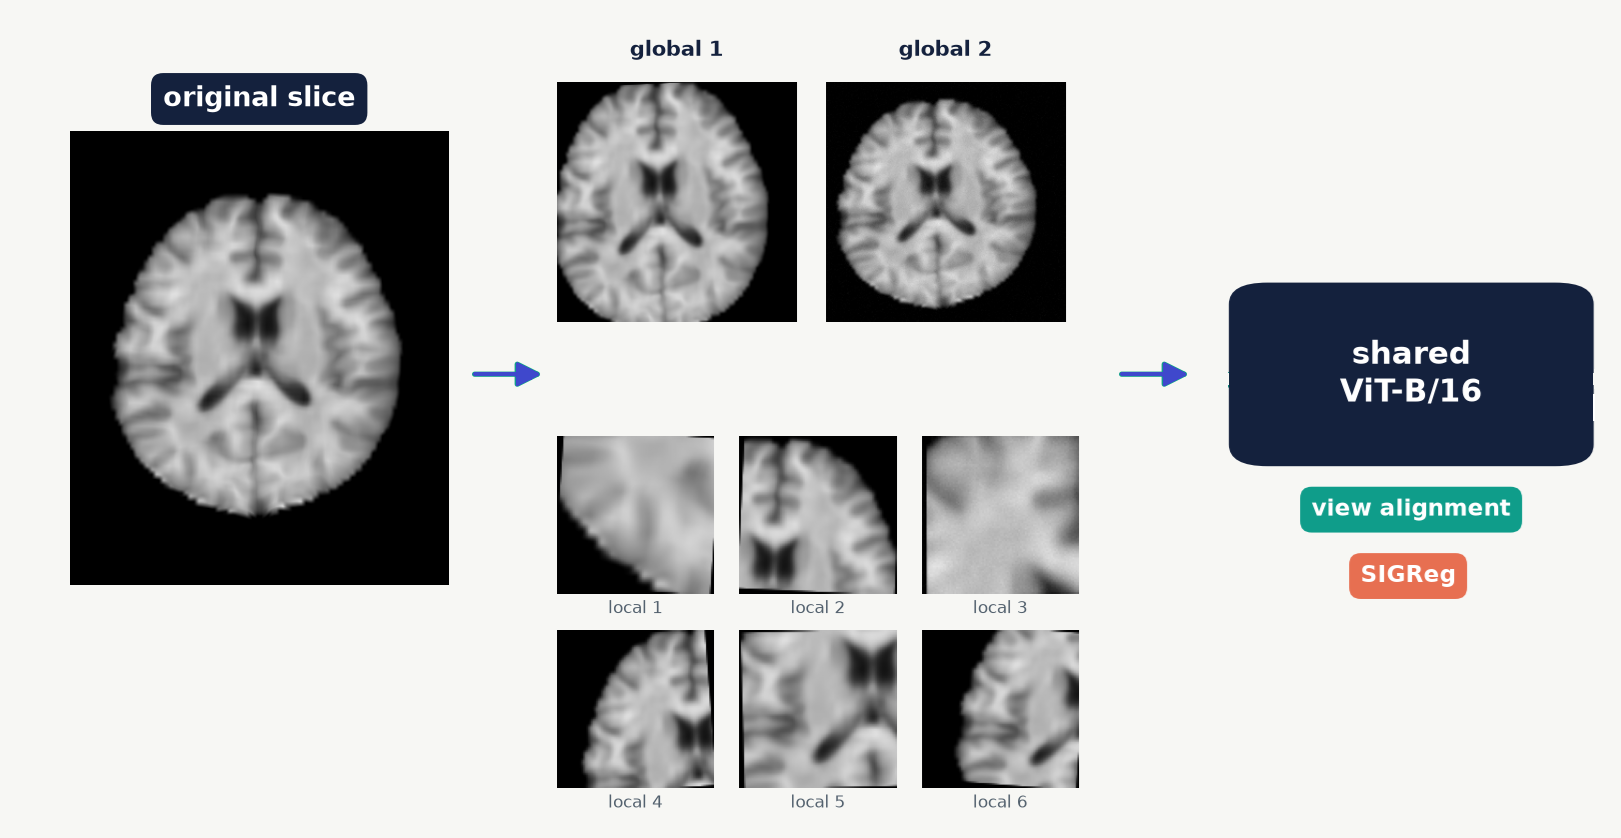
\includegraphics[width=\linewidth]{visuals/02_lejepa_latent_pretraining.png}
  \caption{LeJEPA latent pretraining: multi-crop view generation into a shared ViT-B/16 encoder,
  trained with view alignment and the SIGReg regulariser.}
  \label{fig:lejepa}
\end{figure}

The pretrained encoder was then used to initialise a DPT~\cite{ranftl2021dpt} decoder for Task~1 and compared against a
DINO-initialised~\cite{caron2021dino} and a randomly initialised encoder. Table~\ref{tab:dpt} reports the comparison.

\begin{table}[t]
  \centering
  \small
  \caption{Encoder initialisation ablation, Task 1, T1W only. See the caveat below regarding the other
  two modalities.}
  \label{tab:dpt}
  \begin{tabular}{lccccc}
    \toprule
    Initialisation & \rmse{}~$\downarrow$ & SSIM~$\uparrow$ & LPIPS~$\downarrow$ & Dice~$\uparrow$ & Volume~$\uparrow$ \\
    \midrule
    DPT-DINO   & 0.3760 & \best{0.8806} & \best{0.0865} & 0.8803 & 0.8926 \\
    DPT-LeJEPA & 0.3916 & 0.8783 & 0.0880 & \best{0.8927} & \best{0.9040} \\
    DPT-Random & \best{0.3723} & 0.8796 & 0.0934 & 0.8818 & 0.8909 \\
    \bottomrule
  \end{tabular}
\end{table}

\paragraph{Caveat on this table.} In the experiment log, the T2W and T2FLAIR rows are byte-identical
across all three initialisations, and identical to the corresponding CUT rows. Only T1W differs. We
therefore report T1W alone and treat the modality-averaged figures as unusable pending a re-run. On
T1W the spread is small: $\num{0.0193}$ in \rmse{} and $\num{0.0023}$ in SSIM separate the best and
worst initialisation. Notably, \emph{random} initialisation attains the best \rmse{} of the three while
placing last on LPIPS, and LeJEPA leads on both segmentation-derived metrics while placing last on
\rmse{}. No initialisation dominates, the ordering flips depending on which metric is consulted, and
the whole comparison rests on one modality. We do not consider the question settled.

\section{Conditional U-Net}
\label{sec:unet}

For Task~3 we trained a conditional U-Net directly, as a stronger and much cheaper reference point
than StarGAN~v2. The architecture is standard U-Net, with minor tweaks on blocks; 
each block is two repetitions of $3\times3$ convolution, instance normalisation and LeakyReLU$(0.2)$, 
with $32$ base channels capped at $512$. 
Domain conditioning is deliberately minimal: learned embeddings of the source and target domain
(one of $3 \text{ modalities} \times 5 \text{ field strengths} = 15$) are summed and added to the
bottleneck activation,
\begin{equation}
  h \;\leftarrow\; h + \big(E_{\text{src}}[d_{\text{src}}] + E_{\text{tgt}}[d_{\text{tgt}}]\big),
\end{equation}
broadcast over the spatial dimensions. The output passes through a $1\times1$ convolution and $\tanh$.

The model was trained from scratch for 10 epochs on the prospective training split at
$368 \times 448$ crops, batch size 4, Adam at $10^{-4}$, with mixed precision, under
$\mathcal{L} = \mathcal{L}_1 + 0.05\,\mathcal{L}_{\text{LPIPS}}$. Total loss fell from $0.072$ to
$0.020$.

Despite this modest budget it substantially outperforms the StarGAN~v2 Task~3 baseline on every
reported metric: \rmse{} $0.2364$ versus $0.3436$, SSIM $0.9014$ versus $0.7397$, LPIPS $0.0890$
versus $0.1545$ (Table~\ref{tab:baselines}). Read together with the identity control of
Section~\ref{sec:baselines}, the reasonable interpretation is that a simple regression model with
direct supervision captures the intensity mapping efficiently, and that the adversarial baselines were
paying a large price in stability for no measured benefit.

\section{Spectral analysis}
\label{sec:spectral}

\subsection{Motivation and method}

Dieleman~\cite{dieleman2024} observes that natural image spectra approximately follow a power law, and that because the
Fourier transform is linear, adding white Gaussian noise to an image progressively drowns out its
frequency content from the high-frequency end downward. A diffusion model reversing that corruption is
therefore performing approximate autoregression in frequency space: each denoising step recovers
roughly the next band of frequencies, conditioned on the lower bands already resolved. The strength of
this argument depends entirely on the spectral statistics of the data, so we measured them.

For each axial slice we centre-crop to $364 \times 364$, standardise to zero mean and unit variance,
and compute the radially averaged power spectral density (RAPSD): the squared FFT magnitude, divided
by the sample count, averaged over integer-radius annuli of the shifted spectrum. Frequencies are in
cycles per pixel, so $0.5$ is Nyquist. Standardisation does not affect the fitted exponent (it
shifts $\log P$ by a constant), but it makes curves comparable across field strengths, whose raw
intensity scales differ.

We aggregate the mean of $\log P$ over 12 evenly spaced brain-containing slices per volume and over 30
volumes per cell, and fit
\begin{equation}
  \log P(f) = -\alpha \log f + c
\end{equation}
by least squares, after resampling onto equally spaced log-frequencies so the fit is not dominated by
the high-frequency bins, which are far more numerous. Uncertainty is a percentile bootstrap over
volumes.

\subsection{Choice of fit band}

MRI spectra are not straight lines over the full range, and reporting a single exponent without
qualification would be misleading. Figure~\ref{fig:localslope} plots the local slope
$-\mathrm{d}\log P/\mathrm{d}\log f$. Three regimes are visible. Below $f \approx 0.02$ the spectrum is
dominated by the head-versus-background envelope rather than by tissue texture. Between
$f \approx 0.02$ and $0.2$ the slope is comparatively stable; this is the band carrying anatomical
detail. Above $f \approx 0.2$ every field strength shows a sharp roll-off to local slopes of $5$--$8$,
which is the acquisition and reconstruction band limit, not scene statistics. We fit on
$f \in [0.02, 0.20]$ throughout and shade that band in the figures.

\begin{figure}[H]
  \centering
  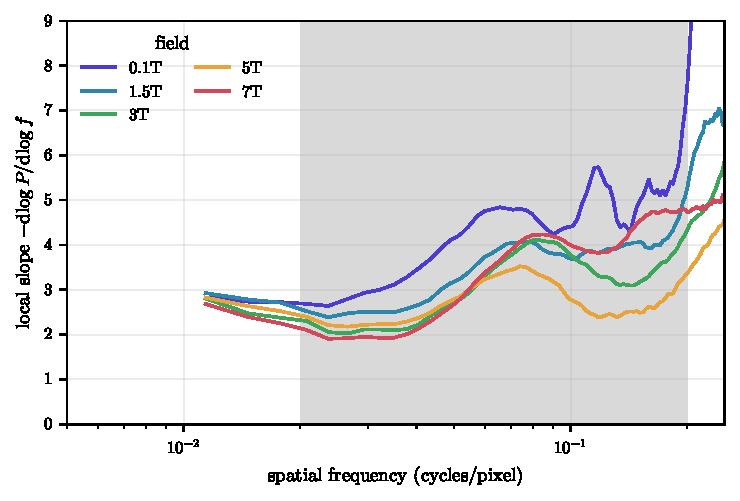
\includegraphics[width=0.62\linewidth]{spectral/fig_local_slope_retro.pdf}
  \caption{Local slope of the log--log spectrum for T1W. A single power law is a reasonable description
  only inside the shaded fitting band; the steep high-frequency region is instrumental roll-off.}
  \label{fig:localslope}
\end{figure}

\subsection{Results}

\begin{table}[t]
  \centering
  \small
  \caption{Fitted spectral exponent $\alpha$ on the training (retrospective) split, estimated over the band $f \in [0.02, 0.20]$ cycles/pixel. Brackets give 95\% bootstrap intervals over volumes ($n = 30$ per cell). Larger $\alpha$ means power falls off faster, i.e.\ relatively less fine detail.}
  \label{tab:alpha-retro}
  \begin{tabular}{lccccc}
    \toprule
    Modality & 0.1T & 1.5T & 3T & 5T & 7T \\
    \midrule
    T1W & \begin{tabular}[t]{@{}c@{}}4.32\\\scriptsize[4.25, 4.38]\end{tabular} & \begin{tabular}[t]{@{}c@{}}3.47\\\scriptsize[3.44, 3.49]\end{tabular} & \begin{tabular}[t]{@{}c@{}}3.14\\\scriptsize[3.12, 3.16]\end{tabular} & \begin{tabular}[t]{@{}c@{}}2.80\\\scriptsize[2.77, 2.83]\end{tabular} & \begin{tabular}[t]{@{}c@{}}3.31\\\scriptsize[3.28, 3.34]\end{tabular} \\
    T2W & \begin{tabular}[t]{@{}c@{}}4.16\\\scriptsize[4.12, 4.21]\end{tabular} & \begin{tabular}[t]{@{}c@{}}2.76\\\scriptsize[2.75, 2.77]\end{tabular} & \begin{tabular}[t]{@{}c@{}}2.60\\\scriptsize[2.58, 2.63]\end{tabular} & \begin{tabular}[t]{@{}c@{}}2.45\\\scriptsize[2.41, 2.48]\end{tabular} & \begin{tabular}[t]{@{}c@{}}2.66\\\scriptsize[2.64, 2.68]\end{tabular} \\
    T2FLAIR & \begin{tabular}[t]{@{}c@{}}3.99\\\scriptsize[3.93, 4.04]\end{tabular} & \begin{tabular}[t]{@{}c@{}}3.04\\\scriptsize[3.02, 3.06]\end{tabular} & \begin{tabular}[t]{@{}c@{}}3.04\\\scriptsize[3.01, 3.06]\end{tabular} & \begin{tabular}[t]{@{}c@{}}2.88\\\scriptsize[2.85, 2.90]\end{tabular} & \begin{tabular}[t]{@{}c@{}}2.69\\\scriptsize[2.68, 2.71]\end{tabular} \\
    \bottomrule
  \end{tabular}
\end{table}


Figure~\ref{fig:rapsd} shows the mean spectra and Table~\ref{tab:alpha-retro} the fitted exponents. Two
observations stand out.

\begin{figure}[t]
  \centering
  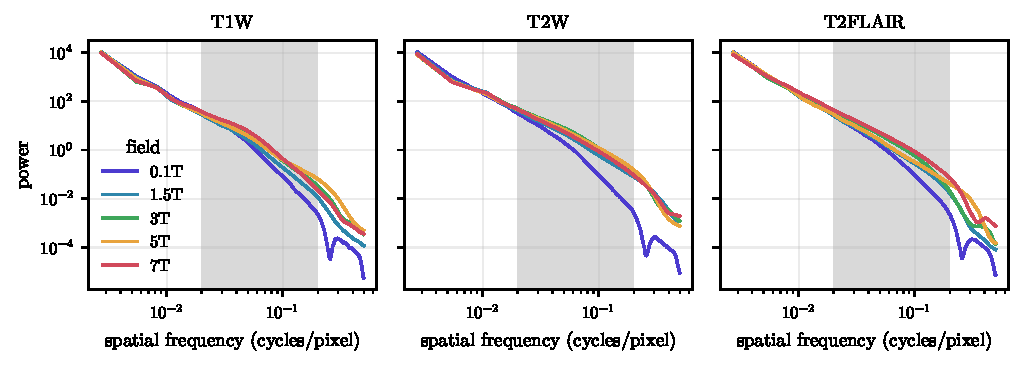
\includegraphics[width=\linewidth]{spectral/fig_rapsd_by_field_retro.pdf}
  \caption{Mean radially averaged power spectra by field strength, one panel per modality
  (retrospective split). The shaded region is the fitting band. In every modality the \SI{0.1}{\tesla}
  curve peels away from the rest above $f \approx 0.03$, while \SIrange{1.5}{7}{\tesla} stay tightly
  clustered: the spectral deficit is specific to \SI{0.1}{\tesla}, not a graded effect of field
  strength.}
  \label{fig:rapsd}
\end{figure}

\paragraph{MRI spectra are steeper than natural image spectra.} Dieleman~\cite{dieleman2024} reports
$\hat{\alpha} \approx 2.45$ for Imagenet, against a canonical value near $2$ for natural images. Our
exponents sit well above that across the board. Brain MRI is a smooth, band-limited, background-dominated
signal with none of the edge and texture statistics that give natural images their heavy high-frequency
tail. A diffusion noise schedule tuned on natural images will consequently spend too much of its
trajectory in a regime where the MRI signal has already been completely masked by noise.

\paragraph{The spectral gap is almost entirely a \SI{0.1}{\tesla} phenomenon.} This is the result that
matters for the challenge, and it is not the smooth trend we initially expected. At \SI{0.1}{\tesla} the
exponent is dramatically larger than at any other field strength: $4.32$, $4.16$ and $3.99$ for T1W,
T2W and T2FLAIR respectively, against a range of roughly $2.4$--$3.5$ for everything else. Between
\SI{1.5}{\tesla} and \SI{7}{\tesla} the differences are small and \emph{not} monotone: $\alpha$ declines
from \SI{1.5}{\tesla} to \SI{5}{\tesla} and then rises again at \SI{7}{\tesla} in T1W ($2.80
\rightarrow 3.31$) and T2W ($2.45 \rightarrow 2.66$), while T2FLAIR continues to decline. We do not have
an account of the \SI{7}{\tesla} upturn; it may reflect acquisition protocol or resolution differences in
that subset rather than tissue contrast, and it is worth checking before it is built upon.

Figure~\ref{fig:fieldgap} shows the same thing as a power ratio to the \SI{7}{\tesla} target and makes
the asymmetry stark. Relative to \SI{7}{\tesla}, the \SI{0.1}{\tesla} deficit grows from nothing at
coarse scales to roughly an order of magnitude by $f = 0.1$; \SI{1.5}{\tesla} sits at a factor of two to
three; \SI{3}{\tesla} is essentially indistinguishable from the target; and \SI{5}{\tesla} carries
\emph{more} high-frequency power than \SI{7}{\tesla} does.

\begin{figure}[t]
  \centering
  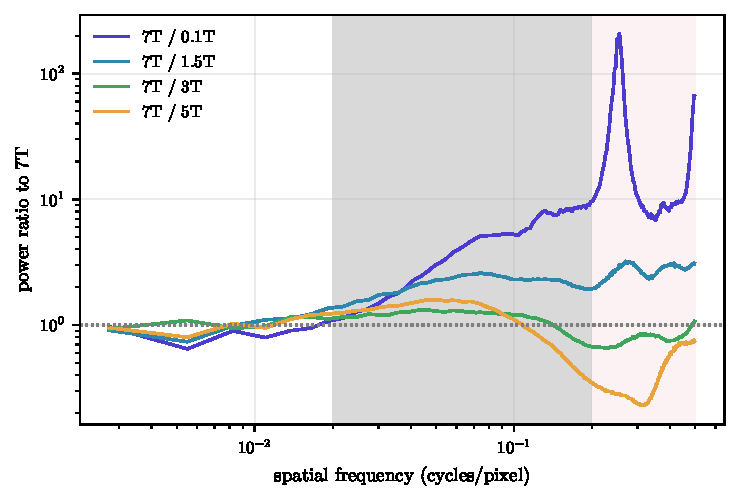
\includegraphics[width=0.62\linewidth]{spectral/fig_field_gap_retro.pdf}
  \caption{Ratio of \SI{7}{\tesla} power to each lower field strength, T1W. Only \SI{0.1}{\tesla}
  shows a large deficit; \SI{3}{\tesla} tracks the target and \SI{5}{\tesla} exceeds it. Grey is the
  fitting band; in the red region both spectra are in instrumental roll-off and the ratio is not
  interpretable.}
  \label{fig:fieldgap}
\end{figure}

\begin{table}[t]
  \centering
  \small
  \caption{Spectral distance to the 7\,T target, $\Delta\alpha = \alpha_{\text{source}} - \alpha_{7\text{T}}$. A positive value means the source is spectrally \emph{steeper} than the target and the model must synthesise high-frequency power that is not present in its input.}
  \label{tab:delta-alpha-retro}
  \begin{tabular}{lcccc}
    \toprule
    Modality & 0.1T & 1.5T & 3T & 5T \\
    \midrule
    T1W & $+1.01$ & $+0.16$ & $-0.17$ & $-0.51$ \\
    T2W & $+1.50$ & $+0.10$ & $-0.06$ & $-0.21$ \\
    T2FLAIR & $+1.29$ & $+0.35$ & $+0.34$ & $+0.18$ \\
    \bottomrule
  \end{tabular}
\end{table}


\subsection{Interpretation: translation as a change of spectral slope}

Combining the two observations gives a compact description of the task. To first order,
\begin{equation}
  \text{translating } B_0 \rightarrow B_0' \quad \text{is} \quad
  P(f) \mapsto P(f)\, f^{-(\alpha' - \alpha)},
\end{equation}
a reweighting of the power spectrum, with the missing power concentrated where the source acquisition
had the least signal to begin with. Table~\ref{tab:delta-alpha-retro} quantifies $\Delta\alpha$ against
the \SI{7}{\tesla} target; note that it is large and positive only in the \SI{0.1}{\tesla} column, and
changes sign at \SI{3}{\tesla} and \SI{5}{\tesla} for T1W and T2W.

This reframes the identity-control result of Section~\ref{sec:baselines}, and the two findings explain
each other. The identity map preserves the source spectrum exactly. For sources at \SI{3}{\tesla} and
\SI{5}{\tesla} that is very nearly the right answer (their spectra already match or exceed the
\SI{7}{\tesla} target across the whole anatomical band), so on Task~1 the identity map is not a
degenerate control at all but a strong one, for three of the four source field strengths. Averaged over
sources, as Table~\ref{tab:baselines} is, this is most of the reason a model that does nothing scores
within noise of models that do something.

It follows that the modality-averaged, field-averaged reporting used so far actively hides the problem.
The only setting with a large spectral gap to close is \SI{0.1}{\tesla}, which is exactly Task~2's
source and one of five sources in Task~1. \textbf{Per-field-strength reporting is therefore not a
refinement but a prerequisite}: a model that solves \SI{0.1}{\tesla}$\rightarrow$\SI{7}{\tesla} and a
model that copies its input are nearly indistinguishable under the current averaged metrics.

\subsection{The connection to diffusion}

Figure~\ref{fig:hinge} reproduces Dieleman's construction~\cite{dieleman2024} on our measured spectra. Adding white noise
of variance $\sigma^2$ to a standardised slice produces the characteristic hinge: the signal spectrum
dominates below the crossing point and the flat noise floor dominates above it. Sweeping $\sigma$ sweeps
that crossing point down through the frequency range. The right panel converts this into the maximal
frequency still detectable at each diffusion time under $\sigma(t) = t/(1-t)$.

\begin{figure}[t]
  \centering
  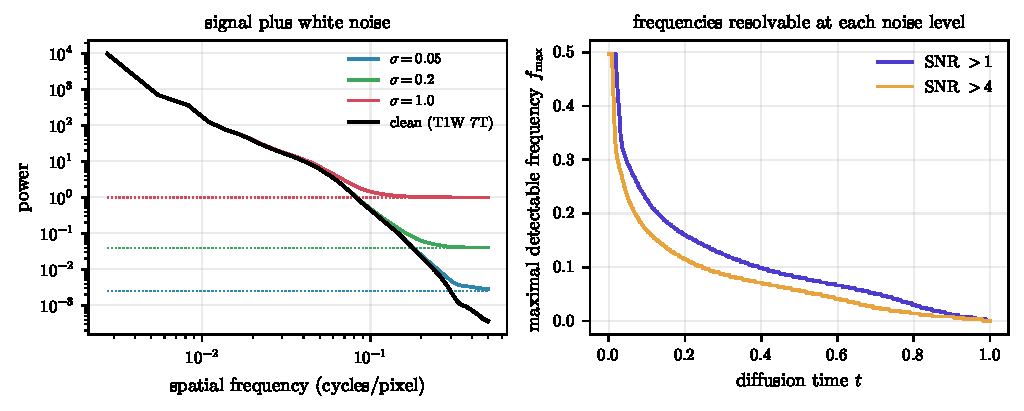
\includegraphics[width=\linewidth]{spectral/fig_noise_hinge_retro.pdf}
  \caption{Left: the measured \SI{7}{\tesla} T1W spectrum with white noise added at three levels,
  showing the hinge. Dotted lines are the noise floors. Right: maximal detectable frequency against
  diffusion time under two SNR thresholds.}
  \label{fig:hinge}
\end{figure}

The practical consequence is that the noise level of a diffusion process indexes a spatial frequency,
and because our exponents are large, that indexing is \emph{steeper} for MRI than for natural images:
a given increment of noise destroys a wider band of frequencies. A schedule imported unchanged from
natural-image diffusion will therefore allocate most of its steps to a regime where nothing remains to
be predicted. This is a concrete, measurable reason to expect off-the-shelf diffusion recipes to
underperform here, and a concrete lever to fix them.

\section{Proposed direction and candidate methods}
\label{sec:direction}

The analysis suggests the target is a model that explicitly controls where in frequency it spends
capacity, conditioned on the source and target field strength. Our intended next step is conditional
diffusion for Task~3, with the noise schedule chosen against the measured spectra rather than inherited.
Candidate directions, in rough order of how well they match what we measured:

\begin{itemize}
  \item \textbf{Frequency-aware diffusion.} Blurring Diffusion Models~\cite{hoogeboom2023blurring} and
  Inverse Heat Dissipation~\cite{rissanen2023ihdm} replace or augment the noising process with an explicitly
  frequency-selective degradation. Given that the task \emph{is} a spectral reweighting, this is the
  most direct match. ``Simple diffusion''~\cite{hoogeboom2023simple} and Chen's noise-schedule
  study~\cite{chen2023noise} give the resolution-dependent schedule adjustment we will need regardless
  of which formulation we pick.

  \item \textbf{Medical-domain precedent.} SynDiff~\cite{ozbey2023syndiff} (adversarial diffusion for unpaired medical image
  translation) is the closest published analogue to this challenge and a sensible reproduction target.
  ResViT~\cite{dalmaz2022resvit} is a reasonable non-diffusion transformer baseline for the same setting.

  \item \textbf{Conditioning mechanism.} The current U-Net's additive bottleneck embedding is the
  weakest part of the design. FiLM-style modulation~\cite{perez2018film}, or classifier-free guidance~\cite{ho2022cfg} over the
  target field strength, would let conditioning act at every scale rather than only at the coarsest one,
  which matters given that the source--target difference is concentrated at fine scales.

  \item \textbf{Representation track.} The LeJEPA encoder work continues in parallel; the natural
  junction is to use the pretrained encoder as the conditioning trunk of the diffusion model rather
  than as a translation backbone in its own right.

  \item \textbf{Field-strength-aware pretraining.} Add a head of five neurons, one per field strength,
  on top of the encoder and train it to predict which field an input came from. After pretraining the
  head is dropped and the encoder is finetuned for translation (Figure~\ref{fig:fshead}). The label is
  free and needs no pairing, so this runs on the unpaired data of Section~\ref{sec:unpaired}. The
  pretraining objective becomes
  \begin{equation}
    \mathcal{L} \;=\; \mathcal{L}_{\text{SSL}} + \lambda\,\mathcal{L}_{B_0},
    \qquad
    \mathcal{L}_{B_0} \;=\; -\log \operatorname{softmax}_{k^\star}\!\big(W z + b\big),
    \quad z = E_\theta(x),
  \end{equation}
  with $W$ of shape $5 \times d$ and $k^\star$ the true field index. The idea is that separating the
  five fields in the latent space gives the translation stage a direction to move along. We would also
  try the regression form $\mathcal{L}_{B_0} = (w^\top z + b - \log B_0)^2$, which keeps the fields in
  their physical order instead of treating them as five unrelated classes.

  Two checks before trusting a result. The head can reach high accuracy on the background floor of
  Section~\ref{sec:background} or on subject identity rather than on field strength, so it should be
  scored with a confusion matrix on masked, renormalised inputs. And our spectral result predicts what
  that matrix looks like if the head is using real signal: \SI{0.1}{\tesla} cleanly separated,
  \SI{1.5}{\tesla} to \SI{7}{\tesla} heavily confused.
\end{itemize}

\begin{figure}[t]
  \centering
  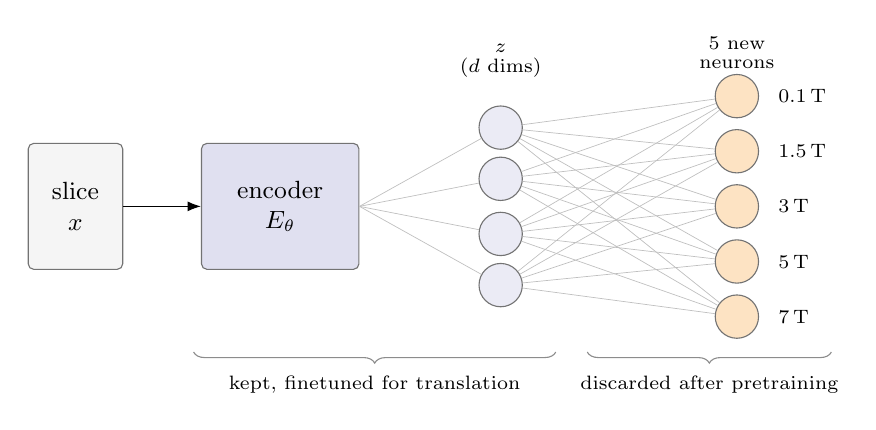
\begin{tikzpicture}[
    >=Latex,
    font=\small,
    unit/.style={circle, draw=black!55, minimum size=5.5mm, inner sep=0pt},
    blk/.style={draw=black!55, rounded corners=2pt, minimum height=16mm, align=center},
    wire/.style={draw=black!25, line width=0.25pt},
  ]
    \node[blk, minimum width=12mm, fill=black!4] (x) at (0,0) {slice\\$x$};
    \node[blk, minimum width=20mm, fill=NavyBlue!12] (enc) at (2.6,0) {encoder\\$E_\theta$};

    \foreach \i/\y in {1/1.0, 2/0.35, 3/-0.35, 4/-1.0}
      \node[unit, fill=NavyBlue!8] (z\i) at (5.4,\y) {};
    \node[font=\scriptsize, align=center] at (5.4,1.85) {$z$\\[-1pt]($d$ dims)};

    \foreach \i/\y/\lab in {1/1.4/{0.1}, 2/0.7/{1.5}, 3/0/{3}, 4/-0.7/{5}, 5/-1.4/{7}} {
      \node[unit, fill=BurntOrange!20] (o\i) at (8.4,\y) {};
      \node[font=\scriptsize, right=1.2mm of o\i] {\lab\,\si{\tesla}};
    }
    \node[font=\scriptsize, align=center] at (8.4,1.95) {5 new\\[-1pt]neurons};

    \foreach \i in {1,...,4}
      \foreach \j in {1,...,5}
        \draw[wire] (z\i) -- (o\j);
    \foreach \i in {1,...,4} \draw[wire] (enc.east) -- (z\i);
    \draw[->] (x) -- (enc);

    \draw[decorate, decoration={brace, amplitude=4pt, mirror}, black!45]
      (1.5,-1.85) -- (6.1,-1.85)
      node[midway, below=5pt, font=\scriptsize, black] {kept, finetuned for translation};
    \draw[decorate, decoration={brace, amplitude=4pt, mirror}, black!45]
      (6.5,-1.85) -- (9.6,-1.85)
      node[midway, below=5pt, font=\scriptsize, black] {discarded after pretraining};
  \end{tikzpicture}
  \caption{Field-strength-aware pretraining. A linear head of five neurons, one per field strength, is
  attached to the encoder output $z$ and trained with cross-entropy against the known field label. The
  head is removed after pretraining; only $E_\theta$ carries over to the translation model.}
  \label{fig:fshead}
\end{figure}

\subsection{UniField: the closest published system}
\label{sec:unifield}

UniField~\cite{lin2026unifield} attacks the same problem as this challenge and is the nearest published
system to what we propose above. It trains a single model for all modalities and both of its field
transitions (\SI{64}{\milli\tesla} to \SI{3}{\tesla}, and \SI{3}{\tesla} to \SI{7}{\tesla}), on the
argument that low-field degradation is shared across modalities and transitions, so joint training acts
as data augmentation. The backbone is latent flow matching inside the frozen encoder and decoder of
FlashVSR, a pretrained \emph{video} super-resolution model, with the volume treated as a video along $z$
and the network adapted by LoRA. Modality and field transition enter as a templated text prompt through
a frozen text encoder (Figure~\ref{fig:unifield}).

The part relevant to us is the Field-Aware Spectral Rectification Mechanism, whose loss is
\begin{equation}
  \mathcal{L}_{\text{FASFL}} \;=\; \lVert v_\theta - v \rVert_1
  \;+\; \lambda_{\text{freq}} \sum_{b \in \mathcal{B}} \frac{w_b}{|M_b|}
  \Big\lVert M_b \odot \big( |F(v_\theta) - F(v)|^{\alpha} \odot |F(v_\theta) - F(v)|^{2} \big) \Big\rVert_1 ,
\end{equation}
with $v_\theta$ the predicted velocity field, $v$ the target, $F$ the FFT, $\odot$ elementwise
multiplication, and $\Delta F = F(v_\theta) - F(v)$ the spectral residual, so the bracket reads
$|\Delta F|^{\alpha} \odot |\Delta F|^{2}$. The bands $\mathcal{B} = \{\text{low}, \text{mid},
\text{high}\}$ are each selected by a binary mask $M_b$, and dividing by $|M_b|$, the number of
frequencies that mask keeps, makes bands of different width comparable. Of the three scalars,
$\lambda_{\text{freq}}$ sets the strength of the spectral term against the spatial $L_1$ term, $\alpha$
controls how sharply the penalty concentrates on the frequencies currently worst fitted, and $w_b$
weights each band.

This is a focal frequency loss ($|\Delta F|^2$ the penalty, $|\Delta F|^{\alpha}$ the reweighting)
restricted to band masks. Written literally the two factors collapse to $|\Delta F|^{\alpha + 2}$; in
the original focal frequency loss the weight $|\Delta F|^{\alpha}$ is detached from the gradient, which
is how we would implement it. What makes it field-aware is that the band weights
$w_b$ are set per transition from a physical argument. At \SI{64}{\milli\tesla} the target's
high-frequency content has no counterpart in the source, so penalising it hard invites hallucination and
the high band is down-weighted; at \SI{7}{\tesla} the targets carry B1 inhomogeneity, which lives at low
frequency, so the low band is down-weighted to stop the model reproducing it. They use
$w_b = [0.2, 0.5, 0.3]$ and $[0.1, 0.3, 0.6]$ respectively, with $\lambda_{\text{freq}} = 0.1$ and
$\alpha = 1$.

\paragraph{What transfers and what does not.} The first term is a per-voxel loss between a prediction
and its own target, so the method needs registered cross-field pairs. Their dataset supplies them, 113
subjects across five centres, registered where the source releases were not; ours does not
(Section~\ref{sec:unpaired}), so UniField cannot be trained on the challenge data as published. Code and
data are announced but not yet released, so this is a read rather than a reproduction for now, and the
paired data is the part we would most want when it lands. Two things transfer regardless. First, the
band weights are hand-set hyperparameters, and Section~\ref{sec:spectral} measures the quantity they
stand in for: $\Delta\alpha$ per transition says which band actually needs weight, so we can derive
$w_b$ from the measured RAPSDs instead of tuning them. The correspondence is not one-to-one, since their
transform is applied to the velocity field in latent space rather than to the image, but the sign and
ordering should carry. Second, their ablation is a useful caution: most of the reported gain comes from
unifying modalities and tasks, with FASRM adding a smaller increment on top.

\begin{figure}[t]
  \centering
  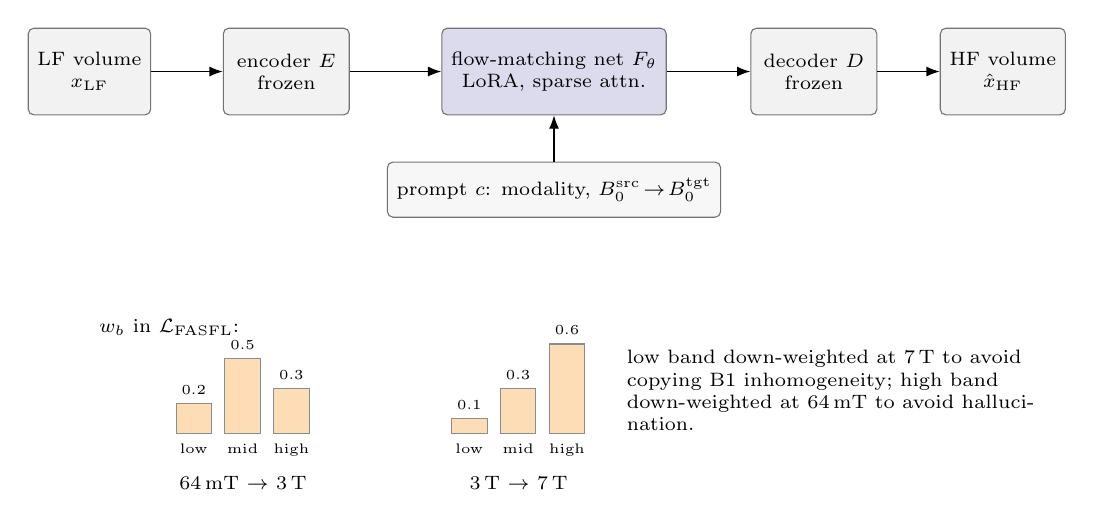
\begin{tikzpicture}[
    >=Latex,
    font=\small,
    blk/.style={draw=black!55, rounded corners=2pt, minimum height=11mm, align=center, font=\scriptsize},
    frozen/.style={blk, fill=black!5},
    train/.style={blk, fill=NavyBlue!14},
    bar/.style={draw=black!45, fill=BurntOrange!25},
  ]
    \node[frozen, minimum width=14mm] (x)   at (0,0)    {LF volume\\$x_{\text{LF}}$};
    \node[frozen, minimum width=16mm] (enc) at (2.5,0)  {encoder $E$\\frozen};
    \node[train,  minimum width=24mm] (net) at (5.9,0)  {flow-matching net $F_\theta$\\LoRA, sparse attn.};
    \node[frozen, minimum width=16mm] (dec) at (9.2,0)  {decoder $D$\\frozen};
    \node[frozen, minimum width=14mm] (y)   at (11.6,0) {HF volume\\$\hat{x}_{\text{HF}}$};

    \foreach \a/\b in {x/enc, enc/net, net/dec, dec/y} \draw[->] (\a) -- (\b);

    \node[blk, fill=black!3, minimum width=34mm, minimum height=7mm] (c) at (5.9,-1.5)
      {prompt $c$: modality, $B_0^{\text{src}} \!\rightarrow\! B_0^{\text{tgt}}$};
    \draw[->] (c) -- (net);

    \begin{scope}[shift={(1.1,-4.6)}]
      \node[font=\scriptsize, anchor=west] at (-1.1,1.35) {$w_b$ in $\mathcal{L}_{\text{FASFL}}$:};
      \foreach \i/\w/\lab in {0/0.2/low, 1/0.5/mid, 2/0.3/high} {
        \draw[bar] (\i*0.62,0) rectangle ++(0.45,\w*1.9);
        \node[font=\tiny] at (\i*0.62+0.225,\w*1.9+0.18) {\w};
        \node[font=\tiny, below] at (\i*0.62+0.225,0) {\lab};
      }
      \node[font=\scriptsize, align=center] at (0.85,-0.62) {\SI{64}{\milli\tesla} $\rightarrow$ \SI{3}{\tesla}};

      \begin{scope}[shift={(3.5,0)}]
        \foreach \i/\w/\lab in {0/0.1/low, 1/0.3/mid, 2/0.6/high} {
          \draw[bar] (\i*0.62,0) rectangle ++(0.45,\w*1.9);
          \node[font=\tiny] at (\i*0.62+0.225,\w*1.9+0.18) {\w};
          \node[font=\tiny, below] at (\i*0.62+0.225,0) {\lab};
        }
        \node[font=\scriptsize, align=center] at (0.85,-0.62) {\SI{3}{\tesla} $\rightarrow$ \SI{7}{\tesla}};
      \end{scope}

      \node[font=\scriptsize, align=left, anchor=west, text width=52mm] at (5.6,0.55)
        {low band down-weighted at \SI{7}{\tesla} to avoid copying B1 inhomogeneity; high band
         down-weighted at \SI{64}{\milli\tesla} to avoid hallucination.};
    \end{scope}
  \end{tikzpicture}
  \caption{UniField, redrawn from the description in~\cite{lin2026unifield}. Top: a low-field volume is
  encoded by a frozen FlashVSR encoder, denoised by a LoRA-adapted flow-matching network conditioned on
  a text prompt naming the modality and the field transition, and decoded by the frozen decoder. Bottom:
  the field-conditioned band weights $w_b$ of the FASFL loss, which are the mechanism's substance.}
  \label{fig:unifield}
\end{figure}

\paragraph{Evaluation.} Given Section~\ref{sec:baselines}, we intend to report a band-limited spectral
error alongside the challenge metrics (the discrepancy between predicted and target RAPSD over
$f \in [0.02, 0.20]$), together with the identity control on every table. Neither is a substitute for
the official metrics, but both make it immediately visible whether a model is doing more than an
intensity remap.

\section{Status and open items}

\begin{itemize}
  \item Baselines for Tasks 1--3 are complete. The competition baselines are treated as a weak
  reference given the identity-control result.
  \item The encoder-initialisation ablation needs re-running on T2W and T2FLAIR; the current log
  contains duplicated rows for those modalities.
  \item The conditional U-Net is a 10-epoch run and has not been tuned; it is a reference point, not a
  submission candidate.
  \item Dice and volume consistency are not yet computed for Task~3.
  \item UniField (Section~\ref{sec:unifield}) is the closest published system to our proposed direction.
  Reproduction waits on its code and paired dataset release; the band-weighted spectral loss can be
  tried on our conditional U-Net before then.
  \item The spectral analysis is complete for the dataset. The corresponding analysis of \emph{model
  outputs}, comparing predicted against target spectra, is the immediate next measurement, and is
  what will show whether any current model recovers high-frequency content at all.
\end{itemize}

\begin{thebibliography}{99}
\small

\bibitem{dieleman2024}
S.~Dieleman. \emph{Diffusion is spectral autoregression}, 2024.
\url{https://sander.ai/2024/09/02/spectral-autoregression.html}

\bibitem{vanderschaaf1996}
A.~van~der~Schaaf, J.~H. van~Hateren. \emph{Modelling the Power Spectra of Natural Images: Statistics
and Information}. Vision Research, 1996.

\bibitem{torralba2003}
A.~Torralba, A.~Oliva. \emph{Statistics of Natural Image Categories}. Network: Computation in Neural
Systems, 2003.

\bibitem{hyvarinen2009}
A.~Hyv\"arinen, J.~Hurri, P.~O. Hoyer. \emph{Natural Image Statistics: A Probabilistic Approach to
Early Computational Vision}. Springer, 2009.

\bibitem{park2020cut}
T.~Park, A.~A. Efros, R.~Zhang, J.-Y. Zhu. \emph{Contrastive Learning for Unpaired Image-to-Image
Translation}. ECCV, 2020.

\bibitem{zhu2017cyclegan}
J.-Y. Zhu, T.~Park, P.~Isola, A.~A. Efros. \emph{Unpaired Image-to-Image Translation using
Cycle-Consistent Adversarial Networks}. ICCV, 2017.

\bibitem{choi2020stargan}
Y.~Choi, Y.~Uh, J.~Yoo, J.-W. Ha. \emph{StarGAN v2: Diverse Image Synthesis for Multiple Domains}.
CVPR, 2020.

\bibitem{billot2023synthseg}
B.~Billot et al. \emph{SynthSeg: Segmentation of brain MRI scans of any contrast and resolution without
retraining}. Medical Image Analysis, 2023.

\bibitem{balestriero2025lejepa}
R.~Balestriero, Y.~LeCun. \emph{LeJEPA: Provable and Scalable Self-Supervised Learning Without the
Heuristics}, 2025.

\bibitem{ranftl2021dpt}
R.~Ranftl, A.~Bochkovskiy, V.~Koltun. \emph{Vision Transformers for Dense Prediction}. ICCV, 2021.

\bibitem{caron2021dino}
M.~Caron et al. \emph{Emerging Properties in Self-Supervised Vision Transformers}. ICCV, 2021.

\bibitem{hoogeboom2023blurring}
E.~Hoogeboom, T.~Salimans. \emph{Blurring Diffusion Models}. ICLR, 2023.

\bibitem{rissanen2023ihdm}
S.~Rissanen, M.~Heinonen, A.~Solin. \emph{Generative Modelling with Inverse Heat Dissipation}.
ICLR, 2023.

\bibitem{hoogeboom2023simple}
E.~Hoogeboom, J.~Heek, T.~Salimans. \emph{simple diffusion: End-to-end diffusion for high resolution
images}. ICML, 2023.

\bibitem{chen2023noise}
T.~Chen. \emph{On the Importance of Noise Scheduling for Diffusion Models}, 2023.

\bibitem{ozbey2023syndiff}
M.~\"Ozbey et al. \emph{Unsupervised Medical Image Translation with Adversarial Diffusion Models}.
IEEE TMI, 2023.

\bibitem{dalmaz2022resvit}
O.~Dalmaz, M.~Yurt, T.~\c{C}ukur. \emph{ResViT: Residual Vision Transformers for Multimodal Medical
Image Synthesis}. IEEE TMI, 2022.

\bibitem{perez2018film}
E.~Perez, F.~Strub, H.~de~Vries, V.~Dumoulin, A.~Courville. \emph{FiLM: Visual Reasoning with a General
Conditioning Layer}. AAAI, 2018.

\bibitem{lin2026unifield}
Y.~Lin, C.~Wang, Z.~Peng, Y.~Yuan. \emph{UniField: A Unified Field-Aware MRI Enhancement Framework}.
MICCAI, 2026. \url{https://arxiv.org/abs/2603.09223}

\bibitem{ho2022cfg}
J.~Ho, T.~Salimans. \emph{Classifier-Free Diffusion Guidance}, 2022.

\end{thebibliography}

\clearpage
\appendix

\section{Validation split spectra}
\label{sec:val-appendix}

The body reports the retrospective split because it is the only one with enough volumes per cell to
support an interval estimate. For completeness, Table~\ref{tab:alpha-val} gives the same fit on the
validation split and Figure~\ref{fig:rapsdval} the corresponding spectra.

\begin{table}[H]
  \centering
  \small
  \caption{Fitted spectral exponent $\alpha$ on the validation (prospective) split, estimated over the band $f \in [0.02, 0.20]$ cycles/pixel. Brackets give 95\% bootstrap intervals over volumes ($n = 3$ per cell). Larger $\alpha$ means power falls off faster, i.e.\ relatively less fine detail.}
  \label{tab:alpha-val}
  \begin{tabular}{lccccc}
    \toprule
    Modality & 0.1T & 1.5T & 3T & 5T & 7T \\
    \midrule
    T1W & \begin{tabular}[t]{@{}c@{}}4.45\\\scriptsize[4.19, 4.61]\end{tabular} & \begin{tabular}[t]{@{}c@{}}3.55\\\scriptsize[3.55, 3.56]\end{tabular} & \begin{tabular}[t]{@{}c@{}}3.26\\\scriptsize[3.22, 3.32]\end{tabular} & \begin{tabular}[t]{@{}c@{}}2.88\\\scriptsize[2.87, 2.90]\end{tabular} & \begin{tabular}[t]{@{}c@{}}3.34\\\scriptsize[3.24, 3.48]\end{tabular} \\
    T2W & \begin{tabular}[t]{@{}c@{}}3.99\\\scriptsize[3.85, 4.14]\end{tabular} & \begin{tabular}[t]{@{}c@{}}3.12\\\scriptsize[3.05, 3.19]\end{tabular} & \begin{tabular}[t]{@{}c@{}}2.91\\\scriptsize[2.76, 3.12]\end{tabular} & \begin{tabular}[t]{@{}c@{}}2.75\\\scriptsize[2.71, 2.77]\end{tabular} & \begin{tabular}[t]{@{}c@{}}3.03\\\scriptsize[3.02, 3.07]\end{tabular} \\
    T2FLAIR & \begin{tabular}[t]{@{}c@{}}3.70\\\scriptsize[3.55, 3.80]\end{tabular} & \begin{tabular}[t]{@{}c@{}}3.32\\\scriptsize[3.30, 3.33]\end{tabular} & \begin{tabular}[t]{@{}c@{}}3.25\\\scriptsize[3.21, 3.27]\end{tabular} & \begin{tabular}[t]{@{}c@{}}3.12\\\scriptsize[3.09, 3.16]\end{tabular} & \begin{tabular}[t]{@{}c@{}}3.34\\\scriptsize[3.33, 3.35]\end{tabular} \\
    \bottomrule
  \end{tabular}
\end{table}


\begin{figure}[H]
  \centering
  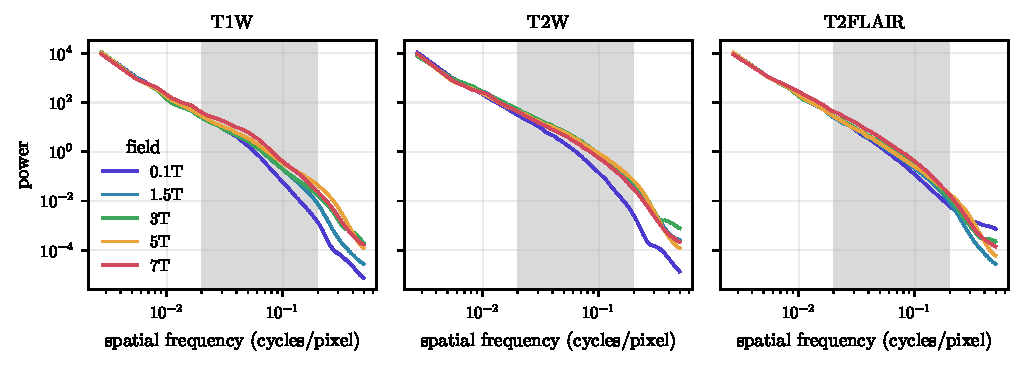
\includegraphics[width=\linewidth]{spectral/fig_rapsd_by_field_val.pdf}
  \caption{Mean radially averaged power spectra by field strength on the validation split
  ($n = 3$ volumes per cell).}
  \label{fig:rapsdval}
\end{figure}

The qualitative picture agrees with the retrospective split, where \SI{0.1}{\tesla} is clearly the steepest
in every modality, but the quantitative agreement is only rough (for example T1W \SI{0.1}{\tesla} is
$4.45$ here against $4.32$ retrospectively, and T2W \SI{1.5}{\tesla} is $3.12$ against $2.76$). The
bootstrap intervals printed for this split should not be read as meaningful: resampling three volumes
cannot characterise between-subject variability, so they are far narrower than the true uncertainty.
Combined with the disjoint-subject structure of Section~\ref{sec:unpaired}, validation-split exponents
are best treated as a consistency check on the retrospective estimates rather than as measurements in
their own right.

\end{document}
